\chapter{Maršrutēšanas protokoli}\label{sec:prot}
Mobilā WSN un Ad Hoc tīklā mezgli nepārtraukti kustās un raida informāciju. Lai atvieglotu maršruta izveides un uzturēšanas procesu tīklā tiek izmantoti maršrutēšanas protokoli. Abiem tīkliem maršrutēšanas protokola mērķis ir ātra un efektīva maršruta izveide un šo uzdevumu ir jāpaveic ar minimālu resursu patēriņu un joslas aizņemšanu. Kā tika minēts \ref{sec:infra} nodaļā, WSN atšķiras no MANET ar to, ka WSN tīklam ir limitēts enerģijas avots, kas arī ir kā uzstādījums un prasība maršrutēšanas protokoliem, taču tas neizslēdz iespēju ka abos tīklos var izmantot vienus un tos pašus protokolus.

Šajā nodaļā ir apskatīti trīs maršrutēšanas protokoli: DSR, AODV un OLSR un nodaļas noslēguma ir piedāvāts maršruta izvēles algoritma optimizācijas veids.

\section{Maršrutēšanas protokolu klasifikācija}
Maršrutēšanas protokolu klasificēšana var tikt izdarīta pēc sekojošiem principiem: \emph{A)} Distances vektora (distance vector) un posma stāvokļa (link state) maršrutēšana, \emph{B)} tabulu vadīta (Table driven) un sūtītāja vadīta (source driven) maršrutēšana un \emph{C)} pēc tīkla topoloģijas veida.

\begin{figure}[ht!]
\centering
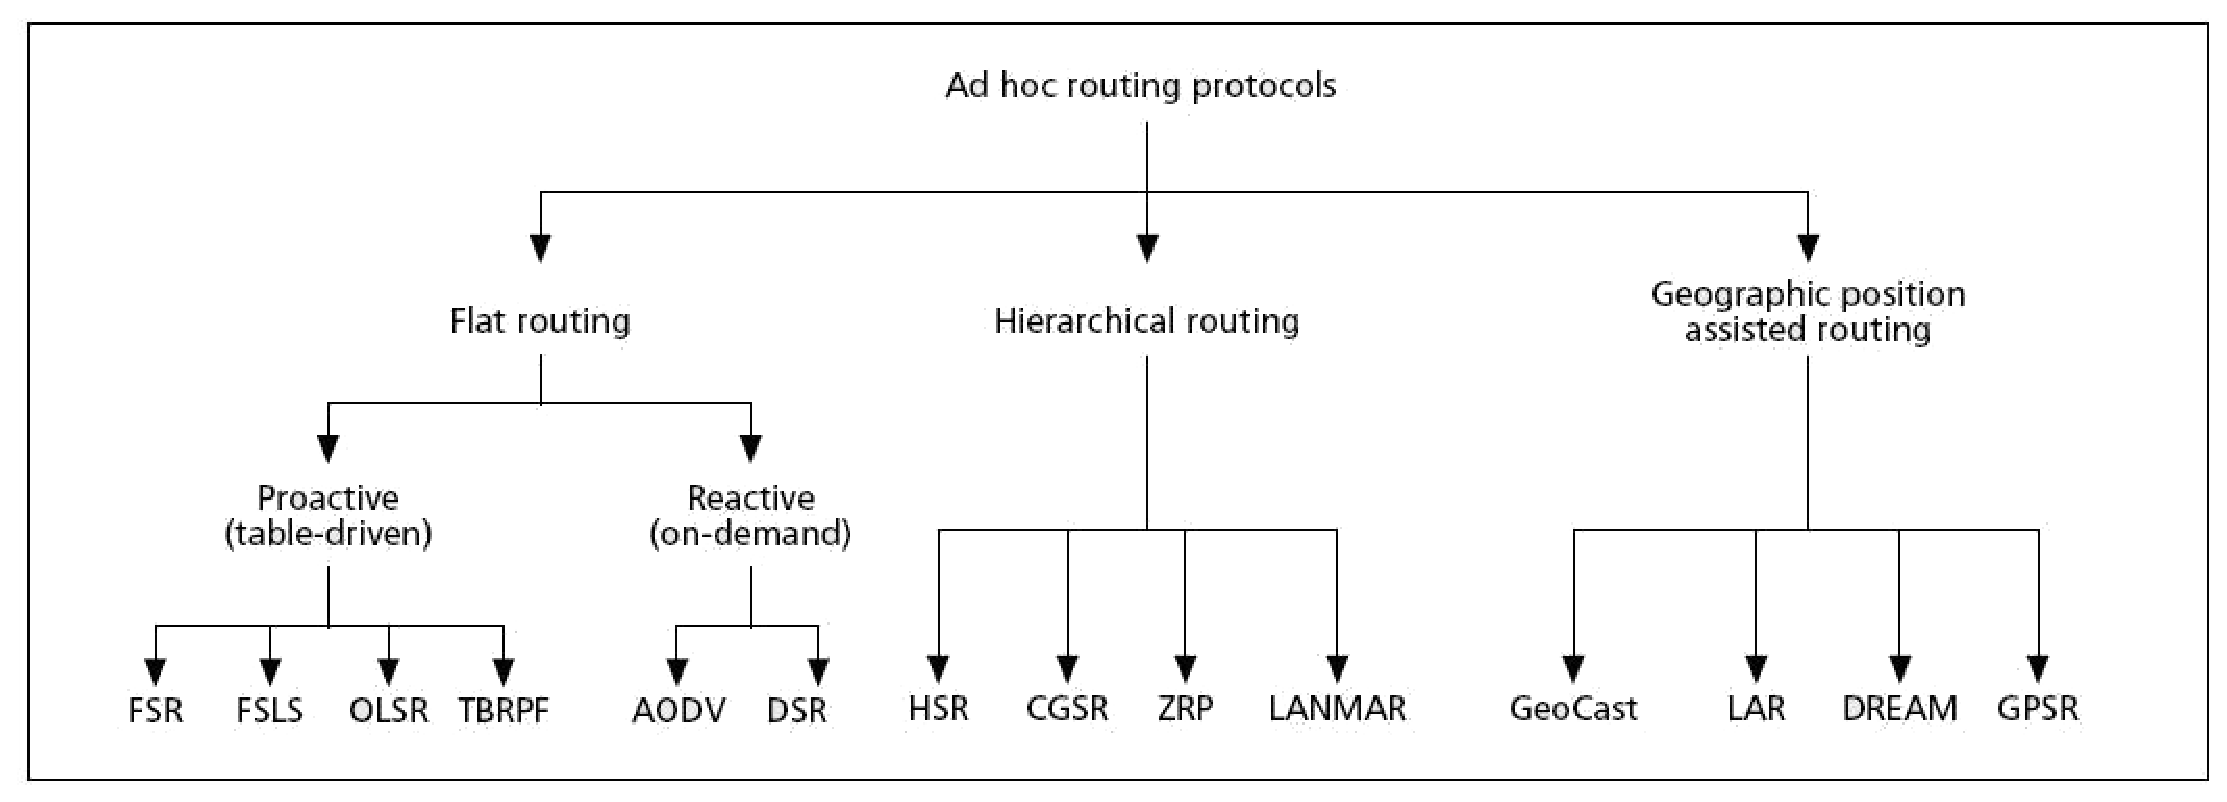
\includegraphics[scale=0.4]{./graph/protocol}
 \caption{Ad Hoc maršrutēšanas protokolu klasifikācija \cite{hong}}
\end{figure}

\textit{Distances vektora}  maršrutēšanas protokols ir balstīts uz decentralizēta algoritma. Katrs tīkla mezgls aprēķina īsāko maršrutu caur tiešiem kaimiņ-mezgliem (pirmās pakāpes kaimiņi) līdz pārējiem tīklā esošiem mezgliem (n-tās pakāpes kaimiņi). Šim maršrutēšanas veidam viens no būtiskākajiem trūkumiem ir: nevienam no mezgliem nav zināma globālā tīkla topoloģija, kā rezultātā ir nepieciešams ilgs laiks līdz visiem tīkla mezgliem ir vienādas ''zināšanas'' par apkārtējo topoloģiju. Att. \ref{fig:rout} a) ilustrē viena lēkuma (one-hop) maršrutu izplatīšanu ar distances vektora protokolu. Mezgla C pārraidītais distances vektors ļauj mezglam B aprēķināt attālumu līdz D kā $B \rightarrow D$ ir 2 un pārraidot šo informāciju A. Savukārt A distances vektors ļauj aprēķināt tā attālumu līdz D kā $A \rightarrow D$ ir 3.

\begin{figure}[ht!]
\centering
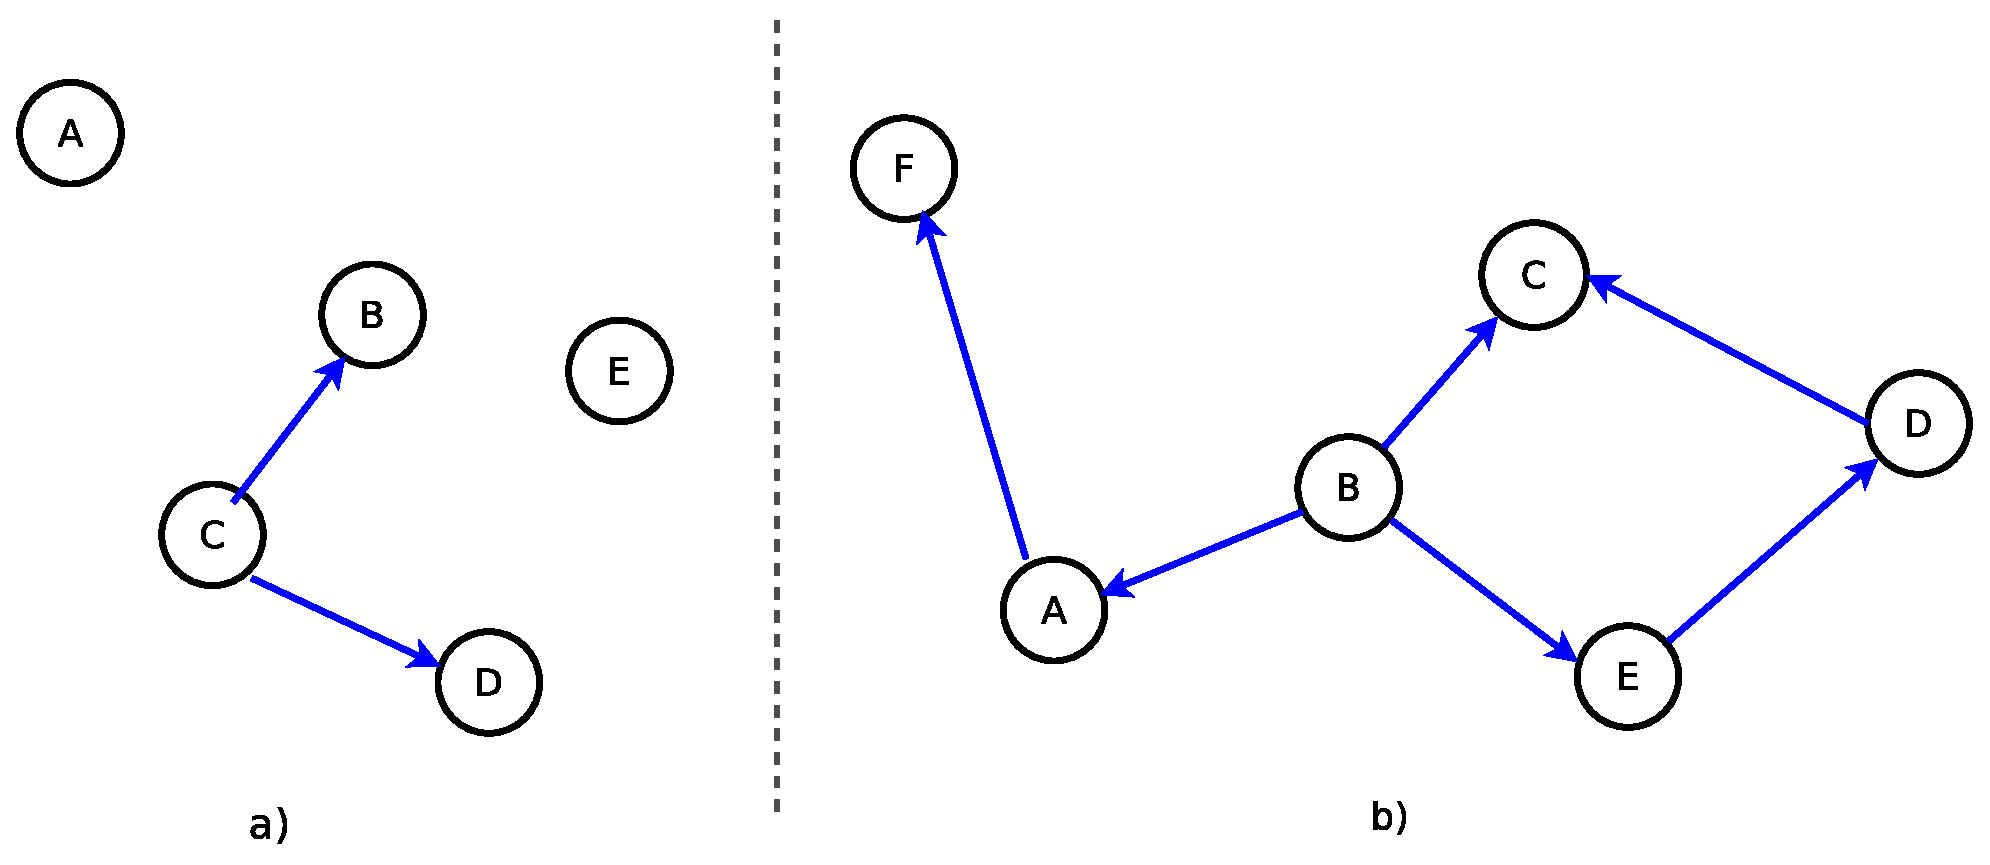
\includegraphics[scale=0.38]{./graph/dis_link}
 \caption{Maršruta atklāšana tīklā ar a) Distances vektora protokolu  un b) Posma stāvokļa protokolu}
\label{fig:rout}
\end{figure}

\textit{Posma stāvokļa} maršrutēšanas protokols balstīts uz globālā maršrutizēšanas algoritma. Katrs tīkla mezgls aprēķina īsāko maršrutu līdz ikvienam tīkla mezglam, tādā veidā iegūstot zināšanas par visiem iespējamajiem maršrutiem. Katrs mezgls pārraida posma stāvokli ikvienam tuvākajam kaimiņ-mezglam lai šī informācija tiktu tālāk pārraidīta visā tīklā. Šāda informācijas apmaiņa ļauj katram tīkla mezglam iegūt informāciju par visa tīkla topoloģiju. Att.\ref{fig:rout} b) ilustrē kaimiņ-mezglu informācijas izplatīšanu, izmantojot pārpludināšanas mehānismu (flooding mechanism). Divas posma stāvokļa paketes, viena no C un otra no B ļauj mezglam A noteikt tā maršrutu līdz mezglam D. \textit{Posma stāvokļa} algoritms salīdzinājumā ar \textit{Distances vektora} algoritmu tiek uzskatīts par labāku risinājumu, jo ļauj izvairīties no ''bezgalīgas skaitīšanas'' (count-to-infinity)\footnote{\emph{count-to-infinity} problēmas. Ja mezgls A informē mezglu B, ka tam ir maršruts līdz kaut kāda veida galamērķim, tad mezglam B nav iespējas uzzināt vai B ir daļa no tā vai nē.} un cilpošanas problēmām.

\textit{Tabulu vadītā} jeb \textit{Proaktīvā} maršrutēšanā. Protokols mēģina secīgi uzkrāt jaunāko informāciju par katru mezglu un izplatīt to katram tīkla mezglam. Protokols katrā mezglā saglabā vienu vai vairākas tabulas ar maršrutu informāciju un protokols reaģē uz tīkla topoloģijas izmaiņām ar atjauninājumu izplatīšanu visā tīklā, lai nodrošinātu konsekventu skatījumu par tīklu. Savā starpā \textit{Tabulu vadītie} protokoli atšķiras ar maršrutēšanai nepieciešamo tabulu skaitu un metodēm ar kurām tiek pārraidītas tīkla struktūras izmaiņas.

\textit{Sūtītāja vadīta} jeb \textit{Pēc pieprasījuma} (On-Demand) maršrutēšana izveido maršrutus tikai tad, kad to pieprasa sūtītāju mezgls. Kad mezglam ir nepieciešams maršruts līdz galamērķim, tas tīklā ierosina maršrutu atklāšanas (route discovery) procesu. Šo procesu var uzskatīt par pabeigtu tikai tādā gadījumā, ja maršruts ir atrasts vai visas iespējamās maršrutu permutācijas ir pārbaudītas.  Kad maršruts ir izveidots, tas tiek uzturēts ar maršrutu uzturēšanas procedūru līdz brīdim, kad galamērķis kļūst nepieejams izmantojot jebkuru no iespējamajiem maršrutiem, vai kamēr maršruta uzturēšana vairs nav nepieciešama.

Tīkla topoloģijas var izdalīt – ar vienotu maršrutēšanu (flat routing), hierarhisku maršrutēšanu (hierarchical routing) un maršrutēšana pēc ģeogrāfiskā izvietojuma (geographic position assisted routing)\cite{hong}. Saskaņā ar tīkla loģiskās struktūras organizēšanas nosacījumiem mobilie Ad Hoc maršrutēšanas protokoli var tik sadalīti uz a) klaster-bāzetiem (cluster-based), b) hierarhisku vai c) vienādranga struktūra, jeb d) hibrīd veida – apvienotā struktūra kas iekļauj abas iepriekš minētos struktūras veidus. Klaster-bāzēti protokoli pēc noteiktas loģikas iedala tīklu klasteros un katram klasterim piešķirot savu galveni. Visas galvenes savstarpēji uztur informāciju par tīkla globālo topoloģiju, šo informāciju galvenes izplata savā klasterī lai nodrošinātu pakešu pārsūtīšanu citiem klastera mezgliem. Vienādranga struktūras tīklā šāda tipa informācija apmaiņa nenotiek, kā rezultātā katram tīkla mezglam kešarmiņā ir jāuztur lokāla maršrutēšanas tabulu.



\section{DSR protokols}\label{sec:dsr}
Dinamiska avota maršrutēšanas protokols (\acs{DSR}) ir avota maršrutēts un maršrutēšanas protokols balstās uz avota iepriekšēju pieprasījumu.  Katrs mezgls kešatmiņā uzglabā maršrutu līdz tam zināmiem mezgliem. Šie dati tiek atjaunoti mezgla kešatmiņā tikai tad, kad tam kļūst zināmi jauni maršruti. Protokolam ir divas galvenās fāzes: maršruta atklāšana (route discovery) un maršruta uzturēšana (route maintenance).

Ja avota mezgls vēlās nosūtīt paketi adresātam, tad tas pārmeklē savu kešatmiņu lai pārliecinātos vai tam jau ir zināms maršruts līdz adresātam. Gadījumā, ja kešatmiņā esošā informācija par maršrutu līdz galamērķim vēl joprojām ir derīga, tad tas izmanto kešatmiņā pieejamo informāciju lai nosūtītu datus. Pretējā gadījumā avota mezgls iniciēs maršruta meklēšanas procesu ar maršruta pieprasījuma paketes (\acs{RREQ}) nosūtīšanu. RREQ satur avota  adresi, galamērķa adresi (varbūt daži) un unikālo idicifišanas numuru. Saņemot RREQ paketi katrs mezgls pārbauda savu kešatmiņu gadījumam vai tam jau ir zināms maršruts līdz galamērķim. Taču - ja starpmezglam nav zināms tāds maršruts, tad tas pievienos savu adresi paketes maršrutu sarakstā (route record) beigās un pārsūtīs to tālāk saviem kaimiņ-mezgliem. Lai ierobežotu RREQ pārsūtīšanas skaitu, mezgls analizē RREQ paketi tikai tādā gadījumā, ja mezgla adrese nav ierakstīta paketes zināmo maršrutu sarakstā. Attēlā ~\ref{fig:dsr} a) pāradīts kā pārvietojas RREQ un izveido maršrutu sarakstu (route record).
\begin{figure}[ht!]
\centering
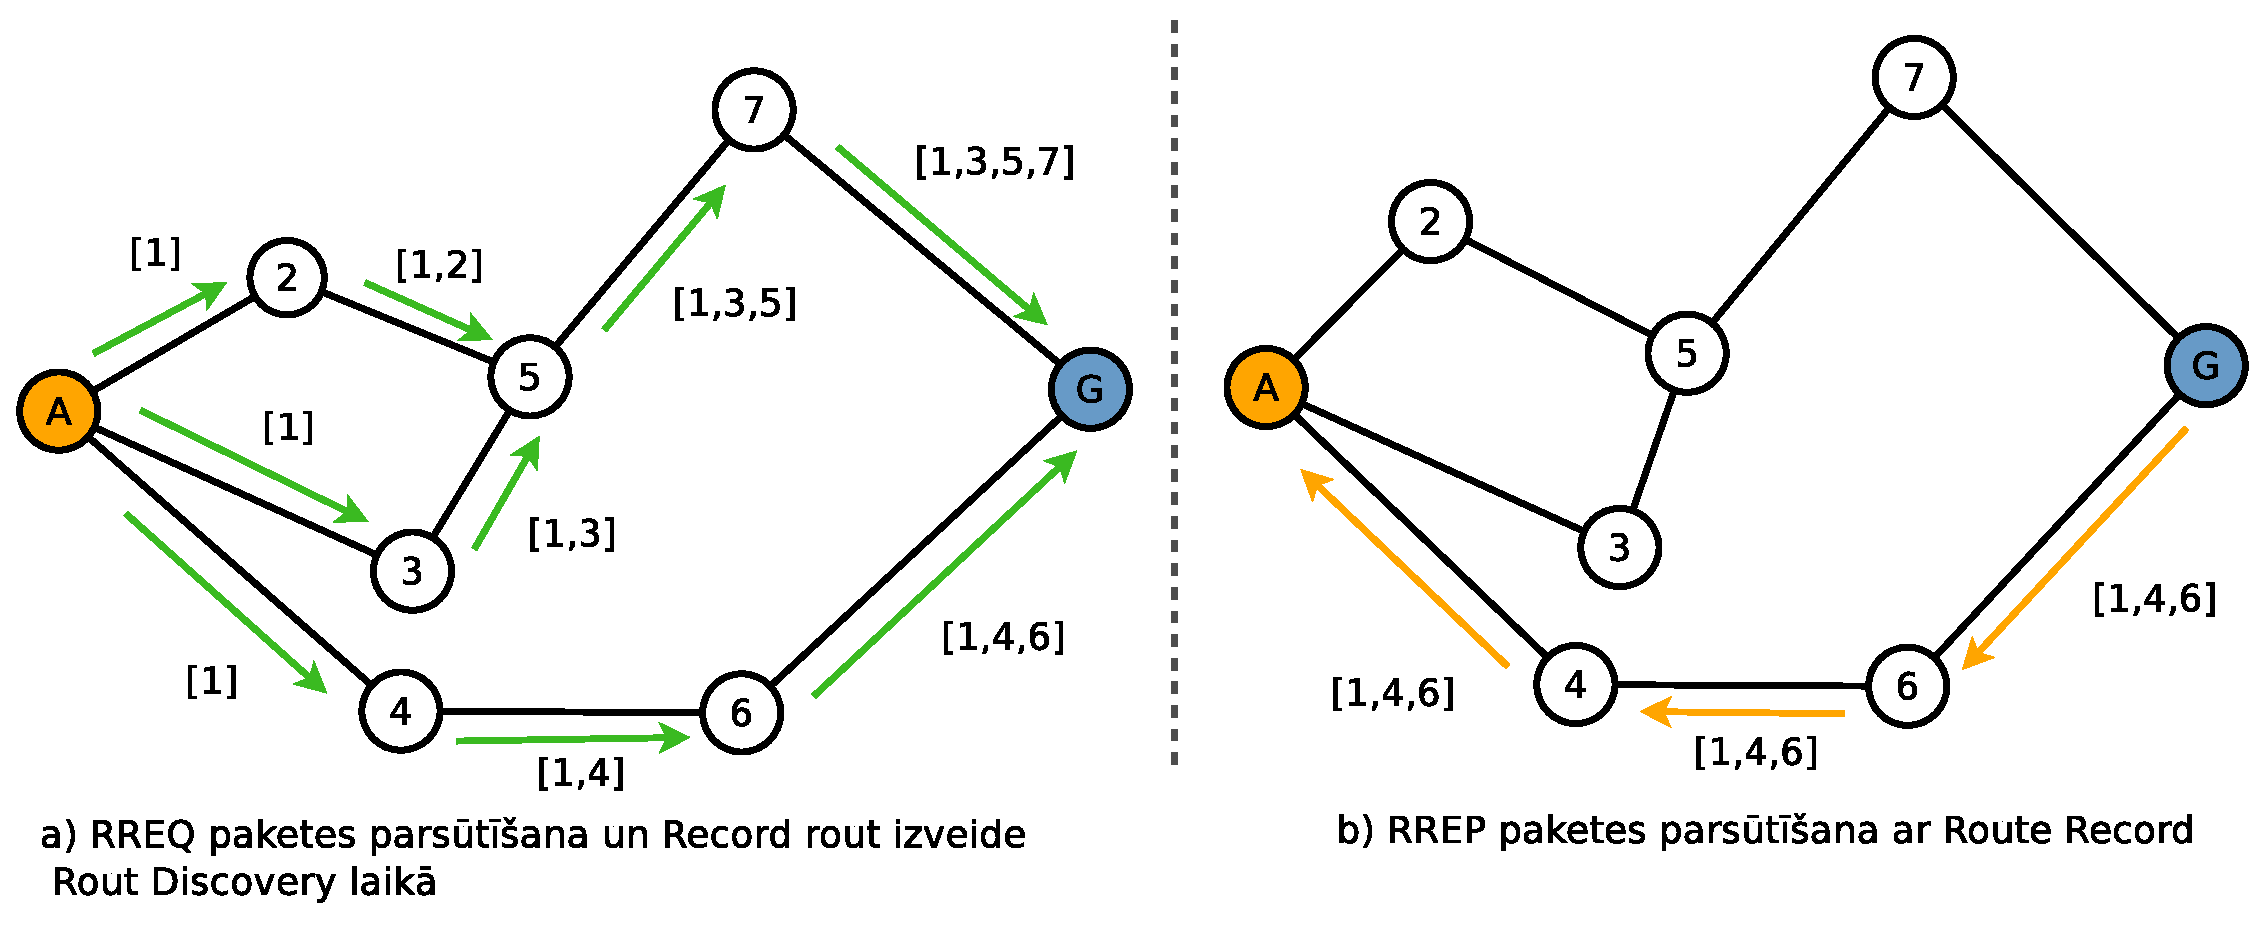
\includegraphics[scale=0.4]{./graph/dsr1}
 \caption{DSR protokola Route discovery}
\label{fig:dsr}
\end{figure}

\acf{RREP}  tiek izveidota ja RREQ sasniedz  galamērķi vai starp mezglu kuram ir informācija par maršrutu līdz galamērķim. Gadījumā ja RREQ sasniedz galamērķi, tad  galamērķis pārkopē maršruta sarakstu (informāciju  par ceļoto maršrutu) no RREQ uz RREP  paketi. Att.~\ref{fig:dsr} b) parādīts ka galamērķis pats nosūta RREP paketi.

Gadījumā kad RREP sasniedz starpmezglu, kuram ir zināma informācija par maršrutu līdz galamērķim, šis mezgls izveido RREP paketi. Mezgls iekopē maršruta sarakstu (route record) no RREQ paketes un pievino to kešatmiņas esošajam maršrutam beigās (RREP = kešatmiņas maršruts + route record). Mezgls var nosūtīt RREP paketi tikai tad, ja tam kešatmiņā ir maršruts līdz avotam. Ja mezglam šādas informācijas nav, tad tas iniciē maršruta atklāšanu (route discovery) līdz pat pašam avotam un pievieno RREP jaunajai RREQ paketei. Maršruta ieraksts (route record) no RREQ paketes var tikt izmantots tikai tādā gadījumā ja tīkla konfigurācija atbalsta divvirzienu savienojumu.

\subsubsection{DSR apkopojums}
DSR priekšrocība ir tā, ka maršruti tiek uzturēti tikai starp tiem mezgliem kas savstarpēji sazinās. Tādēļ paketes virsraksta (header) izmērs pieaug lineāri ar maršruta garumu. Iepriekš minētais, kā arī mezglu kešatmiņas datu aktīvā izmantošana ļauj samazināt virstēriņus, kas ir saistīti ar maršruta uzturēšanu. Tīklos ar DSR maršrutēšanu maršruta pieprasījuma process potenciāli var pārpludināt (flooding) visus tīklā esošos mezglus un kā atbildes reakciju radīt tīklā maršruta atbilžu (RREP pakešu) vēl lielāku pārpludinājumu.

Vēl viens DSR trūkums, ir tas, ka tīklā var rasties cilpas efekts. Gadījumā, ka mezgls izveido RREP balstoties uz savas kešatmiņas datiem. Pastāv iespēja, ka šis maršruts iekļauj sevī iniciējošo mezglu (mezgls kas nosūtīja RREQ). Tāda maršruta izmantošana noved pie cilpas izveidošanas tīklā. Ja tīkla topoloģija ļoti strauji mainās, tas var palielināt virstēriņu dēļ ''novecojušiem'' maršrutu tabulas datiem mezgla kešatmiņā.


\section{AODV protokols}
\acf{AODV} \cite{rfc3561} bija izveidots uz galamērķa secīgā distances vektora protokola (\acs{DSDV}) bāzes 1997.gadā un balstīts uz Bellman Ford algoritma. AODV protokols paredzēts darboties MANET tīklos, kas sastāv no dažiem mezgliem līdz pat tūkstošiem mezglu. AODV raksturiezīmes ir galamērķa secības numurs, IP adresēšana, kā arī tas, ka katrs mezgls izveido maršrutēšanas tabulu. AODV izmanto (\acs{MAC}) protokola beacon paketi lai periodiski pārbaudītu posmu stāvokli ar saviem pirmās kārtas kaimiņiem. Tas palīdz AODV ātri reaģēt uz topoloģijas izmaiņām. Atšķirība no vairākiem MANET protokoliem ir tā, ka AODV var darboties uniraidē un multiraidē. AODV var aizsākt multiraides maršrutēšanu un uzturēt koku kas savieno visus multiraides dalībniekus. Koks sastāv no multiraides dalībniekiem un starpmezgliem.

Galamērķa secības numurs (destination sequence number) kas tiek piešķirts katram ierakstam maršrutēšanas tabulā. Galamērķis izveido un iekļauj secības numuru ikvienā paketē ar maršruta informāciju ko galamērķis nosūta pieprasītajam mezglam (requesting node). Šis numurs ļoti svarīgs, jo tas palīdz mezgliem atšķirt jaunāku maršrutēšanas informāciju (RREQ, RREP) no jau esošajām to tabulām. Galamērķis vai jebkurš starpmezgls var atbildēt uz RREQ. Ja starpmezglam ir zināms maršruts līdz galamērķim, tas nosūta RREP tādā gadījumā, ja tabulā saglabātajai informācijai galamērķa secības numurs ir lielāks par secības numuru RREQ paketē. Galamērķa secības numurs ir izšķirošs lielums gadījumos, kad mezglam ir jāizvēlas starp diviem maršrutiem līdz galamērķim, mezgls vienmēr izvēlas ar lielāku galamērķa secības numuru. Secības numurs ir AODV pamat mehānisms, lai atrisinātu bezgalīgās summēšanas (count-to-infinity) problēmu, kas ir raksturīga visiem distances vektora protokoliem.

Atšķirība no DSR (sk. sadaļa \ref{sec:dsr}), AODV katrā mezglā izveido maršrutēšanas tabulu tādā veidā katrs mezgls uztur vietēju maršrutu kopiju kurā tiek iekļauti dati par to tuvākajiem kaimiņ-mezgliem. Katrs mezgls pārvalda savu posmu stāvokli, kad viens no posmiem tiek pārrauts, mezgls izveido maršruta pieprasījuma error paketes (\acs{RERR}) ziņojumu un nosūta to visiem mezgliem ierakstītiem vietējā tabulā.

AODV ir On-Demand protokols un izveido maršrutus tikai pēc avota pieprasījuma nosūtot maršruta pieprasījuma pakete (\acs{RREQ}) ziņojumu. AODV RREQ ziņojums iekļauj RREQ ID, galamērķa IP adresi, galamērķa secības numuru, avota IP adresi, kā arī avota secības numuru. RREQ ID un avota secības numurs pieaug par vienu katru reizi kad tiek izveidots jauns RREQ. Galamērķa secības numurs ir jaunākais secības numurs ko saņem avots no jebkura cita maršruta līdz šim galamērķim. Ikviens starpmezgls saņemot RREQ saglāba kešatmiņā maršrutu līdz noteiktam RREQ avotam, tādējādi izveidojot atpakaļ ceļu. Kā jau tika minēts, tad ne tikai galamērķis var izveidot RREP ziņojumu, taču RREP ziņojumu var izveidot arī starpmezgls. Proti - ja $dsn_{kesatmina}\geq dsn_{avota}$. galamērķis vai starpmezgls satur derīgu informāciju par maršrutu, tad tas konkrētajam mezglam, kas izveidoja RREQ, var atbildēt uz RREQ ar RREP. Mezgli saglabā šādus datus par RREP: avota ID un tā IP adresi. Tas ir nepieciešams divu iemeslu dēļ. Pirmkārt, lai nogādātu vēlāk sūtītās paketes uz šo galamērķi. Otrkārt, gadījumā ja sūtīts RREP jau vismaz reizi ir ticis pārsūtīts, mezgls to izdzēš - tādā veidā samazinot trafiku. Kad mezgls izveido RREQ/RREP ziņojumu lēkumu skaits ir vienāds ar 0, pārsūtot RREQ/RREP  ziņojumu katrs starpmezgls palielina lēkumu skaitu par 1. Šis mehānisms palīdz starpmezgliem noteikt distanci līdz avotam vai galamērķim izmantotāja maršrutā. Kā arī tas palīdz avotam izvēlēties īsāko maršrutu līdz galamērķim gadījumā, ja ir vairāk nekā viens RREP. Avotam saņemot vairākus RREP ziņojumus, tas tabulā saglabā pirmo ziņojumu un visus nākamos salīdzina ar tabulas ierakstu. Gadījumā ja RREP secības skaitlis ir lielāks vai vienādas un, turklāt, lēkumu skaits ir mazāks par tabulā ierakstīto, tad mezgls tabulā saglabā jauno īsāko maršrutu.
\begin{figure}[!htb]
\centering
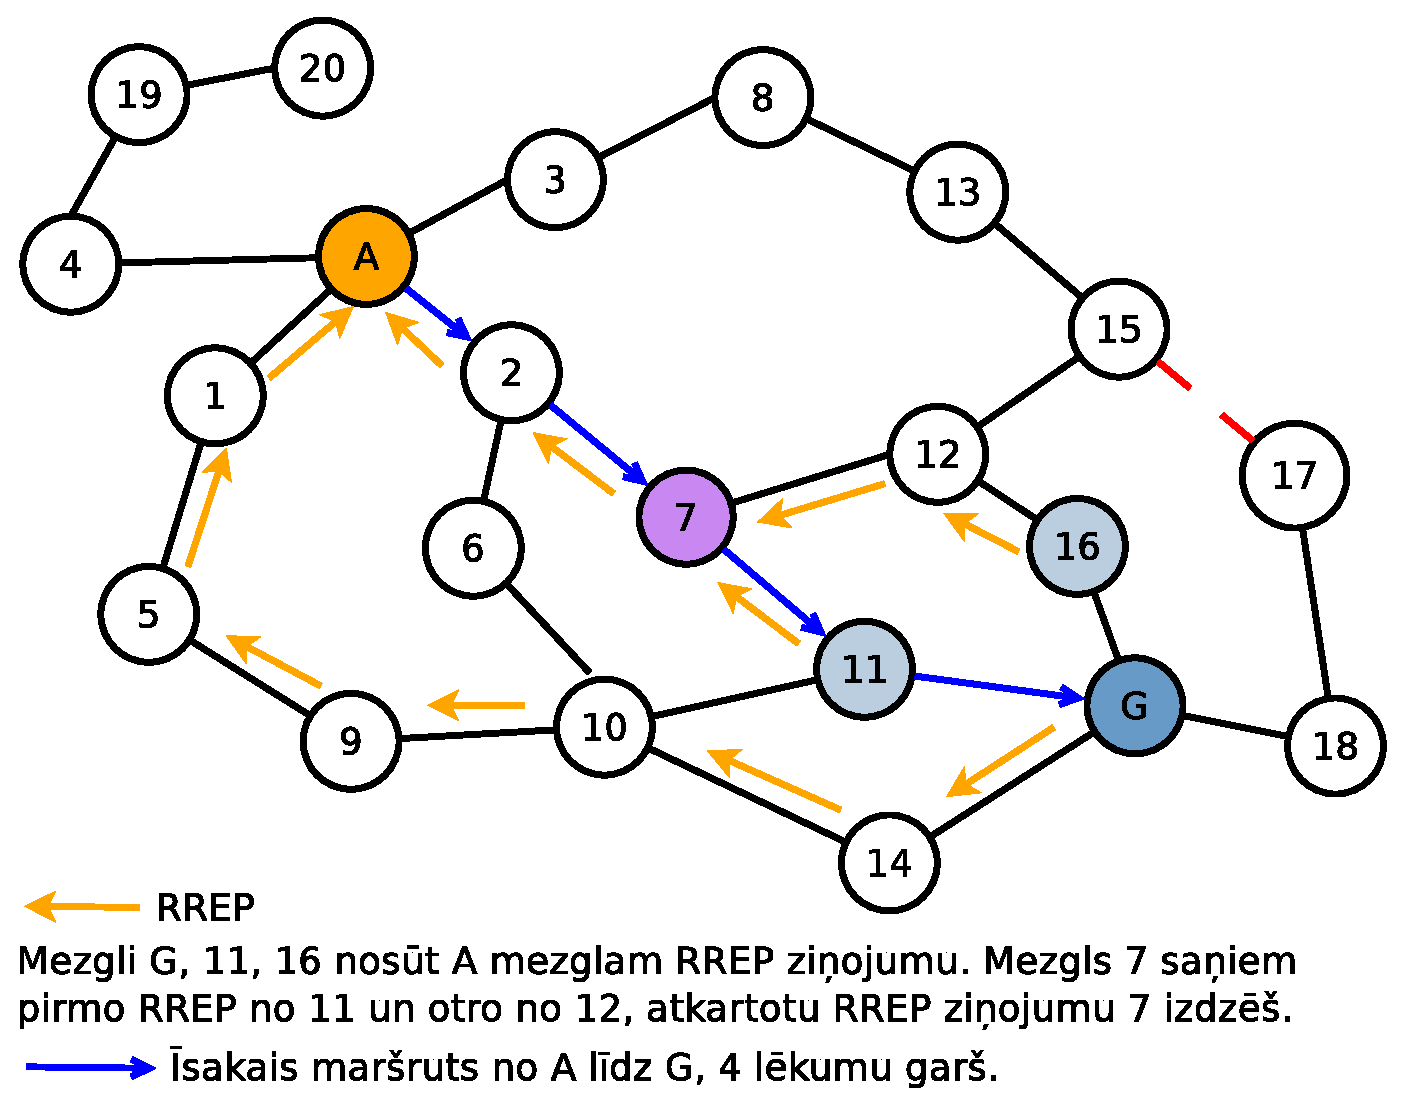
\includegraphics[scale=0.35]{./graph/aodv}
 \caption{AODV protokola datu pārraide tīklā}
\label{fig:aodv}
\end{figure}

Kad maršruts ir izveidots AODV izmanto to tik ilgi cik vien var. Savienojums var tikt izjaukts divu iemeslu dēļ: 1) ja neviens tam nesūta paketes un iestājas noilgums (time-out) un 2) ja kāds no mezgliem iziet no apraides. Ja aktīvi izmantots posms tiek pārtraukts, tad viens no kaimiņ-mezgliem nekavējoties izveido RERR ziņojumu. No maršrutēšanas tabulas mezgls izvēlās mezglus kam maršrutā paredzēts izmantot pārrautu posmu un nosūta tiem RERR. RERR ziņojums sastāv no ''DestCount'', nesasniedzamā galamērķa IP adreses, nesasniedzamā galamērķa kārtas (sequence) numura un galamērķa IP adreses. Kur ''DestCount'' skaits norāda cik galamērķi ir nesasniedzami, nesasniedzamā galamērķa kārtas (sequences) numurs ir kārtas numurs kas tiek ierakstīts mezgla maršrutēšanas tabulā.


AODV izmanto paplašinātu reģiona meklēšanas tehniku (expanding ring search technique), lai kontrolētu pārraides apgabalu. Faktiski, tas palielina dzīvošanas laika (TTL) ilgumu katrā RREQ pārraides kārtā līdz tam brīdim, kad tas saņems RREP. AODV, savukārt, strādā tikai ar simetriskām saitēm.

\subsubsection{AODV apkopojums}
Galvena AODV priekšrocība ir maršrutu izveidošana tikai pēc pieprasījuma. Tas ļauj būtiski samazināt periodisko kontroles ziņojumu virstēriņu, kas ir saistīts ar tabulas vadītu maršrutēšanu. Savukārt, kā trūkumu var minēt to, ka tiek radīta liela pārraides aizture kas ir saistīta ar jauna maršruta atklāšanu. Tas ir tāpēc, ka jaunu maršrutu meklēšanas laikā mezgls ienākošās paketes liek rindā, līdz tiek atrasts jaunais maršruts. Šis ir primārais aspekts, kas rada plūsmas kritumu izteikti mobilos tīklu gadījumos, jo dēļ mainīgas topoloģijas un relatīvi ilga  maršruta izveides laika liels pakešu skaits tiek vienkārši izmests.

\section{OLSR protokols}\label{sec:olsr}
\acf{OLSR} ir proaktīvs maršrutēšanas protokols, kas izveidots uz posma stāvokļa maršrutēšanas protokola bāzes. Klasiskā posma stāvokļa maršrutēšanas protokols  (LSRP) link state pakete satur visu kaimiņ-mezglu sarakstu un ar tiem asociētiem posma izmaksu metrika (link cost metric), kas izraisa lielu kontrolpaketes virstēriņu (overhead). Šis virstēriņš ir šķērslis šaurjoslas tīklos jo pakete tiek piegādāta katram tīklā esošam mezglam (pārpludināt). Padarot pārpludināšanas mehānismu efektīvāku un samazinot kontrolpaketes (contorl packet) virstēriņu jaunais protokols tika nodēvēts par optimizētu posma stāvokļa maršrutēšanas protokolu (\acs{OLSR}).

OLSR samazina atkārtoto pārraižu skaitu izmantojot vairākstāvokļu releju (\acs{MPR}). Tīklā tiek izvēlēti mezgli kas spēj viss efektīvāk pārklāt tīklu, tos dēvē par MPR mezgliem. MPR mezgli ir viena lēkuma (one-hop) kaimiņ-mezgli kuriem ir divvirzienu savienojums un viņi pēc kārtas pārklāj visus divu lēkumu kaimiņus (\figurename. ~\ref{fig:olsr}).

\begin{figure}[!htb]
\centering
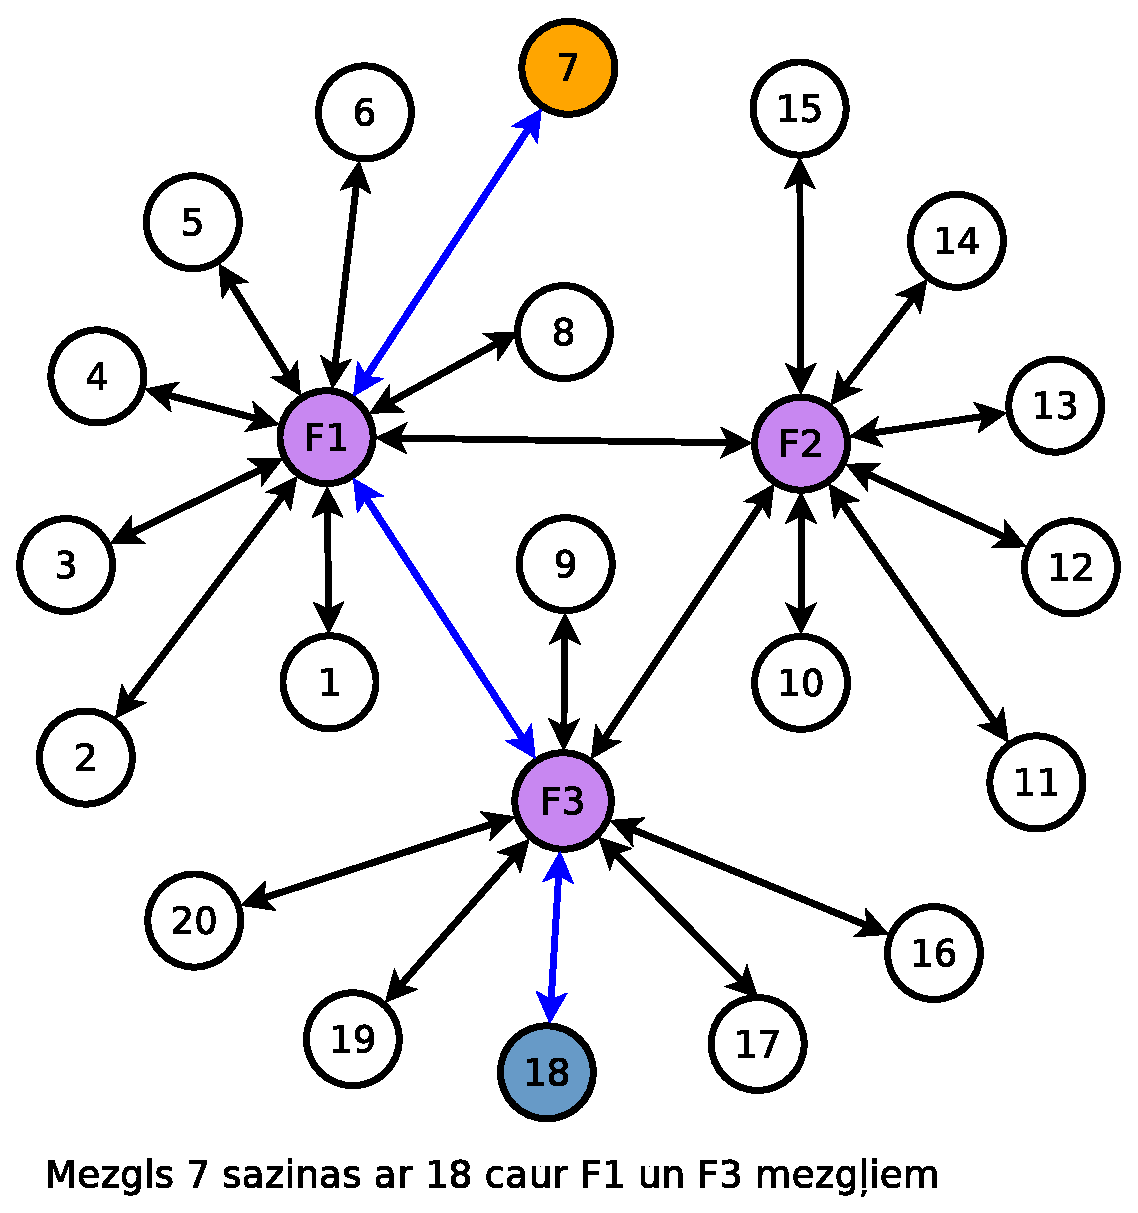
\includegraphics[scale=0.35]{./graph/olsr}
\caption{Datu pārraide tīklā ar OLSR protokolu}
\label{fig:olsr}
\end{figure}

Tīklā ar OLSR protokolu visi mezgli tiek iedalīti divās grupās: 1) MPRset (\figurename. ~\ref{fig:olsr} apzīmēti ar F1, F2, F3) un 2) MPRselctorset. Kur MPRset sastāv no izvēlētiem MPR mezgliem un MPRselectorset ir mezglu grupa, kuriem izvēlētais mezgls ir MPR mezgls. MPR mezgla izvēlētā grupa (MPRselectorset) darbojas kā pārsūtīšanas stacijas - tās saņem ienākošos datus un pārsūta tos uz galamērķi savā MPRselectorset. Šis paņēmiens palīdz samazināt virstēriņa posma statusa (link state) paketes, jo tikai MPR posma stāvokļa kontrolpaketē ir iekļauta posma stāvokļa statusā (link state connectivity) informācija.

Sākumā mezgli savu darbību uzsāk ar tukšām MPRset un MPRselectorset tabulām. Katrs mezgls izvēlas grupu no kaimiņ-mezgliem, tā lai katrs otrais kaimiņ-mezgls būtu sasniedzams ar šīs grupas starpniecību. OLSR izmanto vienkāršu zondēšanas shēmu lai atklātu kaimiņ-mezglu posma (link) statusu. Kaimiņmezglu posma statusam ir trīs iespējamās stadijas: vienvirziena (unidirectional), abu virzienu (bidirectional) un MPR. Periodiski OLSR izplata HELLO ziņojumu - šajā ziņojumā tiek iekļauti nesen komunicēto kaimiņ-mezglu saraksts un to posma statusi (link state). Kad mezgls saņem HELLO ziņojumu tas atzīmē posmu kā vienvirziena (unidirectional) lokālajā kaimiņ-mezglu tabulā un nākamajā HELLO ziņojumā iekļauj tajā sava kaimiņ-mezgla identifikatoru - ID. Kad kaimiņ-mezgls saņem šo HELLO ziņojumu ar savu ID tas atzīmē šo posmu kā abpusēju (bidirectional). Katrs mezgls izmanto dalītās aproksimācijas algoritmu (distributed approximation algorithm) lai izrēķinātu savu MPRset un marķē posmu ar šo mezglu kā MPR savā lokālajā tabulā.

RFC 3626  sadaļā 8.3.1, ir detalizēti aprakstīts heiristisks algoritms MPRset izrēķināšanai \cite{rfc3626}. HELLO ziņojumi tiek pārraidīti noteiktā MPRselctorset zonā, tādējādi samazinot joslas izmantošanu. No HELLO ziņojuma mezgli uzzina kas bija izvēlēts kā MPR mezgls. Saņemot HELLO ziņojumu MPR mezgls atzīmē sūtītāju savā MPRselectorset sarakstā. Visa tīkla posma statusa (link state) informācijas apmaņa notiek ar Topoloģijas uzraudzības ziņojumu (\acs{TC}). Periodiski katrs MPR mezgls tīklā pārraida pārējiem MPR mezgliem TC ziņojumu, kas satur MPR mezgla ID un tā MPRselectorset sarakstu. Šeit ir arī svarīgi atzīmēt, ka šādu ziņojumu sūta ne tikai tie MPR mezgli, kuriem MPRselectorset saraksts nav tukšs. Pamatojoties uz TC ziņojumu informāciju, mezgli var aprēķināt īsāko ceļu līdz katram mezglam tīklā. Ir svarīgi arī saprast, ka OLSR maršruts vienmēr iekļauj MPR mezglus kā retranslācijas punktu. Tāpēc OLSR maršruts nav iespējamais īsākais maršruts tīklā.

\subsubsection{OLSR apkopojums}
OLSR priekšrocība ir tā, ka šis protokols samazina kontroles informācijas apjomu un tādējādi izteikti samazina nepieciešamo trafika apjomu pārraidāmajā joslā. Lai arī OLSR iekļauj informāciju par katru maršruta posmu no avota līdz galamērķim, tas nebūt nenozīmē, ka piedāvātais maršruts ir visīsākais, jo notiek datu retranslācija caur MPR mezglu. Kā vēl vienu no OLSR protokola trūkumiem var minēt to, ka MPR mezglos, kad tie operē kā lokalizēti retranslējoši mezgli, ir novērojama maršrutēšanas aizture kā arī joslas virstēriņš. Tomēr, saskaņā ar protokola specifikāciju \cite{rfc3626}, OLSR uzrāda labus rezultātus ļoti blīvā tīklā ar augstu RWM mezglu kustību.

\section{Maršruta izvēles algoritma optimizācija}\label{sec:BERSP}
Šajā nodaļā apskatītie protokoli izmanto Bellman Ford algoritmu maršruta izvēlei, gadījumiem kad līdz vienam galamērķim ir pieejami vairāki maršruti. Izvēle tiek izdarīta vadoties pēc kopējā maršruta garuma, izvēloties visīsāko maršrutu (short-path). Īsākais maršruts nodrošina ātrāku datu pārraidi, bet tas ne vienmēr nozīmē arī visaugstāko servisa kvalitāti (QoS). \acl{QoS} tīklā ir atkarīga no bitu kļūdu intensitātes (\acs{BER}), datu pārraides ātruma un datu aizkavēm pārraides laikā. Ja maršrutēšanas protokols izvēlas maršrutu pēc Bellman Ford algoritma principa, tas, pirmkārt, mazina potenciālo datu aizkaves laiku un, otrkārt, saskaņā ar formulu (\ref{eq:BER_route}) (\seename \ref{sec:BER} sadaļu) mazinās $BER_{route}$, pie nosacījuma ka visos maršrutos $BER_{link}$ ir viens un tas pats. Taču jāņem vērā, ka mainīgas topoloģijas gadījumā šis nosacījumus nav iespējams.

Pēdējā laikā daži pētnieki piedāvā aizvietot Bellman-Ford algoritmu ar jauniem BER-bāzētiem algoritmiem \cite{olsr_ber} un \cite{qoS_static}.  T.Yelemou un P.Meseure savā darbā piedāvā BER-balstītu MPR izvēlētu OLSR maršrutēšanas protokolu \cite{olsr_ber}. Kā arī G.Ferrai un O.Tonguz \cite{qoS_static} piedāvā RESGO MAC BER-bāzētu protokolu, kas izvēlas maršrutu balstoties uz BER līmeni galamērķī. Tāds paņēmiens palīdz nodrošināt zemu BER līmeni, taču šis ieguvums, savukārt, tiek sasniegts ar maršruta garuma pieaugumu \cite{qoS_static}.

Abiem algoritmiem ir trūkumi un savas priekšrocības, lai mazinātu trūkumus šai maģistra darbā tiek  apskatīta iespēja apvienot šos algoritmus vienā algoritmā. Jaunais BER-SP algoritms ir balstīts uz kompromisu starp BER līmeni un posmu skaitu maršrutā. Tas izvēlas maršrutu ar īsāko maršrutu no saraksta kuram $BER_{route}$ ir zemāk par $BER_{app}$. Kur $BER_{app}$ ir BER līmenis kuru nepieciešams  nodrošināt pareizai lietojumprogrammas darbībai.  Algoritma darbība var tikt aprakstīta sekojošā veidā:
\begin{center}
 \begin{verbatim}
 1. Atrast visus zināmos maršrutus līdz galamērķim N
 2. Ja maršrutu skaits ir lielāk par 1, tad
     2.a No maršrutu saraksta izvēlēties vienu ar vissmazāko mezglu skaitu
     2.b Salidzīnāt izvēlētā maršruta BERroute ar BERapp
     2.c Ja  BERroute <= BERapp izvēleties šo maršrutu
     2.d Ja  BERroute > BERapp atkārtot procesu parējiem maršrutiem
 3. Ja otrajā solī netika izvelēts neviens maršruts
    3.a No saraksta izvēlēties maršrutu ar vismazāko BERroute
\end{verbatim}
\end{center}
Lai skaitliski pamatotu šī algoritma veiktspēju, izmantojot MATLAB tika simulēta SP, BER-bāzētu un BER-SP darbība izmantojot gadījuma lielumu $BER_{route}$ un $n_{h}$. Līdz vienam galamērķim ir 7 iespējami maršruti [$BER_{link}$ $n_{h}$], no šiem maršrutiem SP, BER-bāzēts vai SP-BER izvēlas vienu kas ''vislabāk'' atbilst algoritmu kritērijam. Programma izpilda 50 iterācijas lai izslēgtu nejaušības (MATLABa kodu skatīt \ref{appen:matlabSPBER}).

\begin{figure}
 \centering
 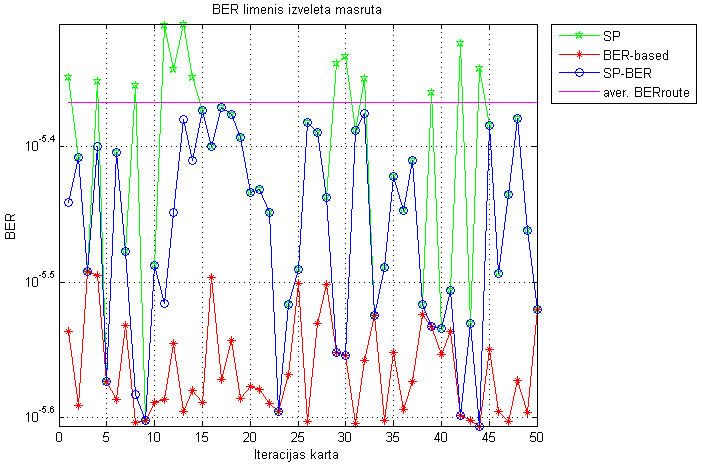
\includegraphics[scale=0.75]{./graph/BERSP_BER}
\caption{Dažādu algoritmu BER līmenis izēvelētajā maršrutā}
\label{fig:SPBER_ber}
\end{figure}

Attēlā \ref{fig:SPBER_ber} pāradīts BER līmenis izvēlētajā maršrutā atkarībā no maršrutēšanas algoritma. Uz Y ass izvietotas BER vērtības algoritmu izvēlētajā maršrutā un uz X ass iterācijas kārtas numurs. Salīdzinājumā ar SP algoritmu (attēlā zaļā krāsā) BER-SP (attēlā zilā krāsā) parāda labākus rezultātus, ko arī varējām gaidīt.
\begin{figure}[!htb]
 \centering
 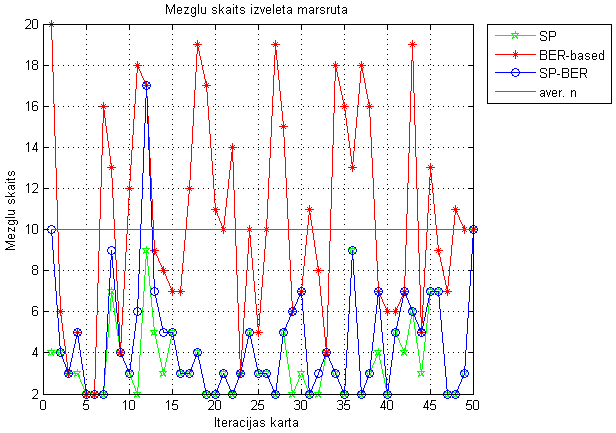
\includegraphics[scale=0.75]{./graph/BERSP_n}
\caption{Dažādu algoritmu posmu skaits izvēlētajā maršrutā}
\label{fig:SPBER_rho}
\end{figure}

Attēlā \ref{fig:SPBER_rho} pāradīts posmu skaits izvēlētajā maršrutā atkarībā no maršrutēšanas algoritma. Kā arī tika paredzēts, ka BER-bāzēta posmu skaits ir viss augstākais salīdzinājumā ar pārējo algoritmu izvēlētajiem maršrutiem. Savukārt BER-SP izvēlētajos maršrutos (attēlā zilā krāsā) vairākumā no posmu skaita kas ir mazāks par vidējo mezglu skaitu $n_{h}$(rozā līnija).

Šeit ir jāatzīmē, ka ir svarīgi noteikt pareizo $BER_{app}$ līmeni. Gadījumā kad $BER_{route}$ $\gg$ $BER_{app}$ BER-SP darbosies kā BER-bāzēts algoritms un izvēlēsies maršrutu ar viszemāko $BER_{route}$. Savukārt gadījumā, kad $BER_{route}$ $\ll$ $BER_{app}$ tas darbosies pēc SP algoritma principa, izvēloties visīsāko maršrutu jo visiem maršrutiem $BER_{route}$ ir zemāks par $BER_{app}$.

Maģistra dara izstrādes laikā nespēju atrast nevienu zinātnisku publikāciju, kas aprakstītu šādu maršrutēšanas algoritmu.